\chapter{Community-Led OurPlace Engagements}
\label{chap:Community}

The original research path of the OurPlace project can be split into two branches: investigating how the application can be used as a seamless, place-based learning tool within formal education contexts; and how it can be used as a platform for civic learning, with place stakeholders sharing knowledge and values to meet their own agendas. This chapter focuses on engagements which meet the latter, describing an multiyear ethnographic study with a local heritage group and the engagements which came as a result of it. 

The work covered by Section \ref{sec:TalkingStatue} was part of a body of work which was peer-reviewed and published at MobileHCI 2018 \citep{Richardson2018}, with the paper being co-authored by Doctors Pradthana Jarusriboonchai, Kyle Montague and Ahmed Kharrufa.

\subsubsection{For clarity}
During the early engagements covered in this chapter, the OurPlace platform was still called `ParkLearn', and lacked the Follow-Up Tasks functionality. Otherwise, the apps were functionally very similar---see Chapter \ref{chap:Design} for more information. The rebranding of ParkLearn to OurPlace occurred in response to findings covered in Section \ref{sec:HeritageParkLearnWorkshop}.

\section{Creating a Talking Statue using ParkLearn}
\label{sec:TalkingStatue}

Two members (male and female, aged in their 60s) of a local park's volunteer group approached the Parks2026 (discussed in Section \ref{sec:Parks2026}) research group, following engagements unrelated to this project. They had seen the Talking Statues project \citep{Sing2017}, and wanted to produce their own version for their park. This original version used QR codes to launch a mobile-friendly website, where celebrity narrations would inform the user about the history of the statue and the local area. The volunteers wanted to make their own version, built upon an existing monument of a key figure of their park's history. They wanted this `talking statue' to share his story with visitors, encourage them to further explore the park and even to join the volunteer group. However, as the volunteers had very limited technical knowledge and funds, a bespoke digital technology (in the same vein as the original Talking Statues project) seemed inaccessible to them. A physically wired system would have also been too expensive, and would also have interfered with the monument’s status as a listed historical structure. They had hoped that our research group would see this as an opportunity to create a new research project. When this didn't happen, I recognised that the newly expanded ParkLearn app was a viable alternative.

I met with the volunteers at their park, to introduce them to the ParkLearn app and discuss what they would want out of the project. While they were satisfied with the app's functionality, they were most taken by the lack of infrastructure needed by the app, and the potential speed of its deployment: they had previously anticipated the installation to take over a year to develop and deploy, whereas the ParkLearn Activity could be ready almost immediately. Furthermore, they were very surprised by the lack of cost---something which was a major concern, as the volunteer group existed on a shoestring budget. With these reasons in mind, the volunteers decided to create the installation using the app. This was to be the first deployment of ParkLearn `in the wild'.

While the process of creating an Activity can be completed in only a couple of minutes, the talking statue took several weeks to prepare. This was partly down to the need to decide upon and generate content: the volunteers needed to write a script for what the statue should say, and also decide on what else should be included in the Activity. Several drafts were written, balancing the desire to add historical detail with the need to keep the audio recordings short and accessible. The volunteers also considered ways in which they could advertise their volunteer group to interested visitors---as well as inform learners about the park's history, they also wanted to spread awareness of their group's efforts, and how it could be supported. Finally, the volunteers also needed to decide how the Activity should be accessed by visitors. They decided that in order to access the Activity, the user should have to be at the statue in person. This meant that the Activity would have to be set to private, with QR Code scan points provided at the statue itself. Another factor which delayed the deployment was that the volunteers applied for funding from the local council to print Foamex signs, which would be stronger and more weather resistant than laminated paper. They also required permission from the council to feature these signs semi-permanently in the park.

\begin{figure*}
  \centering
  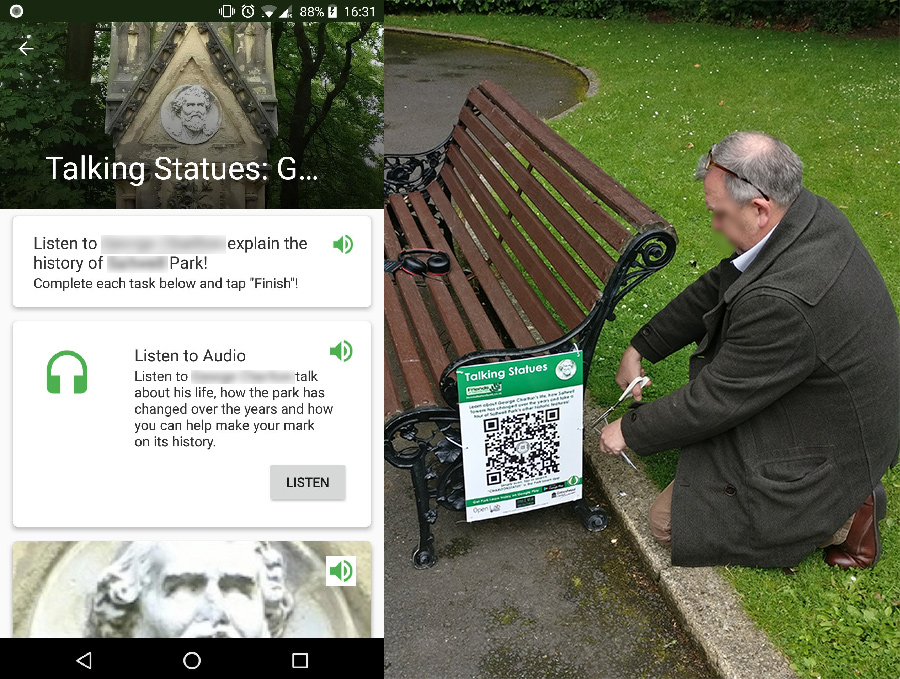
\includegraphics[width=0.8\columnwidth]{images/chapter06/TalkingStatue2.jpg}
  \caption[The ParkLearn `Talking Statue' Activity, and installing the signage ]{Left to right: A) The `Talking Statue' ParkLearn Activity. B) The male park volunteer installing Foamex signs featuring the Activity's QR code.}~\label{fig:TalkingStatueActivity}
\end{figure*}

The final `talking statue' Activity was created at the female volunteer's house, with my help (while both had a base level of digital literacy, neither were hugely comfortable with using new technologies). The Activity featured a narration of the park's history from the perspective of the statue, written and read by the male volunteer. This was recorded directly into the app for a \textit{Listen to Audio} Task (Figure \ref{fig:TalkingStatueActivity}.A). The volunteers were keen for a written transcript of the narration to also be included, so that the Activity would be accessible to those who are hard of hearing. To this end, the speech was transcribed using \textit{Information} Tasks, which also featured historical photos of the park and external links to the volunteer group's website. Finally, the Activity used \textit{Location Hunt} Tasks to guide the learner to the park's eight listed structures (unfortunately as ParkLearn lacked Follow-Up Tasks, no additional content could be unlocked upon arrival).

The Foamex signs were printed with a simple design featuring the Activity's QR code (supplied by the ParkLearn website), and attached to benches near the statue using zip ties (Figure \ref{fig:TalkingStatueActivity}.B). By making the Activity ‘private’ and using these signs, the volunteers could ensure that only people near the statue could launch the Activity. As this meant people would have to be present in the park to use it, they treated the statue as an attraction, something that would raise the profile of the park and encourage people to visit. They printed posters to advertise the project to the surrounding community, and even talked to the local press. 

\begin{figure*}
  \centering
  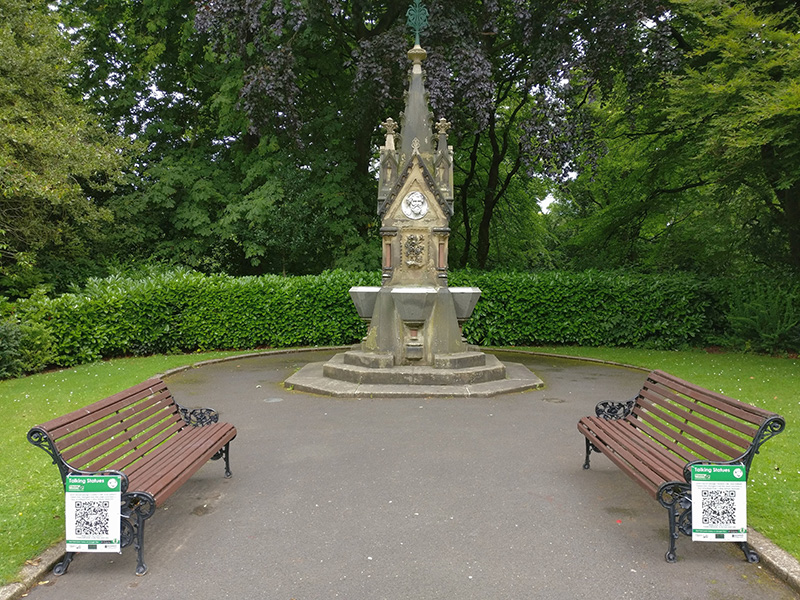
\includegraphics[width=0.85\columnwidth]{images/chapter06/TalkingStatue.jpg}
  \caption[The ParkLearn `Talking Statue' installation]{The final ParkLearn `Talking Statue' installation.}~\label{fig:TalkingStatue}
\end{figure*}

After the launch of the installation, the volunteers were eager for regular updates regarding its usage by park visitors. To facilitate, I updated the ParkLearn website to show the number of times each Activity had been scanned (95 scans in the first 30 days). They were proud of the installation, and demoed it to several volunteer groups from other parks in the area. The signs are still in place over two years later (although one was stolen, and had to be replaced), with around 1200 scans logged.

ParkLearn allowed the volunteers to create a digital, multimedia instalment with minimal interaction or support from the local council (from whom they required permission to put up the scan points). Due to the use of pre-existing technology, the total cost of the installation was around £50 (the cost of producing the signs). The talking statue launched in the same summer in which it was conceived, rather than the original target launch date of the following year. With assistance from the researcher, the actual creation of the Activity took less than an hour.

\section{An Ethnography within the Heritage Forum}

Following the success of the Talking Statue, I was invited to attend a meeting of a grassroots heritage group (referred to from here on by the pseudonym `Heritage Forum', or `HF') which was being hosted in the park. The male park volunteer was a member of this forum, and wanted to thank me for enabling the talking statue project and introduce me to the other members. This meeting spawned a several-year relationship with the Heritage Forum.

\subsection{An Overview of the Heritage Forum}
The Heritage Forum was formed in 2015 by representatives of local heritage groups active within the North-East of England, and exists as an alliance of key heritage bodies and individuals active within the region. The HF is volunteer-based, and exists as a registered charity. Motivated by austerity politics restricting the amount of public funding dedicated to the protection and preservation of heritage, the Forum celebrates that the region was at the forefront of world development during the period of the Industrial Revolution, and `\textit{seeks to make a tangible and significant impact on the regional environment to the benefit of those who live and work there}'.

The Forum is particularly focused on the heritage surrounding the period of the Industrial Revolution, a time of technical innovation and intense population and economic growth during the \nth{18} and \nth{19} centuries. The North-East of England at this time was recognised for being extremely influential in terms of new technologies: notable figures from the region include George Stephenson (who built the world's first public inter-city railway line), Joseph Swan (invented the incandescent light bulb, with Newcastle boasting to have the first street to be lit by electric light) and William Armstrong (an industrialist whose house featured the world's first hydroelectric power station). The region also has a significant industrial heritage, particularly surrounding shipbuilding, glass production, coal mining and iron, steel and chemical manufacturing. 

The HF performs several functions. They have organised several conferences, which are attended by local heritage community groups and institutions, history enthusiasts, historians and representatives from local government. These conferences feature heritage-related keynote speakers, presentations, interactive workshops, stalls and opportunities for groups to network. The Forum also runs an initiative which provides advice, mentorship and practical support to local heritage groups. The initiative's marketing material notes:

\begin{displayquote}
"We can provide advice and support for heritage and history groups wishing to better understand, protect and improve access to a historic structure or place in their community, as well as mentoring in areas such as project development, understanding significance, conservation, understanding statutory and planning frameworks, applying for funding, setting up a charity, developing partnerships, creating interpretation, learning programmes and more."
\end{displayquote}

The Forum is largely made up of working and retired professionals (including architects and town planners), history enthusiasts and academics. The numbers of members in regular attendance vary, with typically between 5-12 attending the monthly meetings. While the majority of members who were retirees and history enthusiasts were male (and obviously of retirement age), the working professionals skewed largely female, with most in their twenties and thirties. However, the main figures (e.g. the Chair) of the Forum, and the individuals most likely to attend every meeting, were male.

\subsection{Reflections on Working within the Heritage Forum}
As a result of the talking statue project, I was invited to hold a `workshop' about my work at the Heritage Forum's 2017 conference. While this was labelled as a workshop, it actually consisted of a slot within a series of guest presentations/lectures. When feedback from many conference attendees suggested a greater emphasis on interactivity, the Forum asked if I would like to host a full interactive workshop, due to my prior experience in running such workshops for research. The details of this workshop---and a discussion of the findings that came of it---are covered in Section \ref{sec:HeritageParkLearnWorkshop}.

Following this workshop, I gradually became a more permanent member of the Forum, attending the monthly meetings and several social events over the course of the next two years. These meetings generally consisted of members discussing progress that they had made in respect to heritage projects they themselves are engaging with (for example, one member was coordinating with the local council to create a publicly accessible area around an old water well). Due to the nature of volunteer work and the levels of bureaucracy involved with local authorities and planning permission, progress tended to be slow with nearly all projects that the Forum engaged with (the well project had started underway when I first joined the group, and at the time of writing still only exists on paper). 

As well as covering progress on members' projects, these meetings also concerned the organisation of the Forum's public events, including workshops and conferences. As well as the workshop discussed in Section \ref{sec:HeritageParkLearnWorkshop}, I helped plan and run a public Heritage Forum workshop aimed at how volunteer groups could better utilise social media for engagement (delivered by a colleague as a part of their research project relating to community volunteer groups' usage of social media platforms); assisted in the organisation of the Forum's 2018 conference (which I helped restructure to support the existence of longer, interactive workshops); ran a short workshop at this conference (discussed in Section \ref{sec:HeritageOurPlaceWorkshop}; and helped the group move towards holding smaller and more regular `Meetup' style engagements, rather than large annual conferences.

This move towards smaller, more frequent community engagements was prompted by the recognition of how much of the  responsibility of organising the conferences had been placed on relatively few members. Towards the end of my engagements with the Forum, I had noticed that several of the members---particularly these few---had started showing signs of weariness of the Forum: partly due to the tasks involved in organising its engagements, but also born of frustration with the group's lack of progress and tendency to quibble on minutia, without making lasting decisions. I believe this may be a reason for why the `Talking Statue' project appealed to them: the ParkLearn app allowed individual members to take action and create an installation, with little need for prolonged engagement with bureaucratic institutions such as the Forum or local authorities.

The Heritage Forum exists as an interesting case study when viewed under the lens of the impact of David Cameron's `Big Society' policies (discussed in Section \ref{sec:DigitalCivics}). The group formed out of a perceived necessity for civic action to protect and develop artefacts of the North East's heritage, due to a lack of investment from local government. The Forum's existence could actually be viewed as the Localism Act working as intended---local community members coming together through volunteerism, sharing their expertise to assist others in effecting local societal change. The Forum's services, which utilise and share their gathered specialist knowledge, somewhat counteract the issues faced with regards to citizens not having the skills or domain knowledge to put the Localism Act to effective use \citep{BBCSundayPolitics2013}, and how the government haven't provided the resources or opportunities for self-education \citep{BenRogers2010a}. However, many of the other issues surrounding having a reliance on volunteerism still remain---active participation in the Forum is somewhat gated by the necessity of having the free time to do so, inadvertently resulting in a membership largely relying on age and/or privilege (I saw no people of colour attend Forum meetings). Thus, the only community voices able to effect change in local heritage through the Forum were those who could afford to volunteer their time to do so. While there was an active push within the Forum to get more young people involved, there didn't seem to be much reflection about other aspects of diversity and representation. While it may be unfair to hold volunteer groups to the same diversity standards as employers (they aren't going to turn down willing volunteers, and can't force anyone of particular demographics \textit{to} volunteer), the resulting underrepresentation is the same: something which could potentially be easier to mitigate if publicly funded, due to a lessened reliance upon volunteerism.

Furthermore, the fatigue that several members were experiencing may point towards a lack of sustainability with self-organised community groups of this kind. The volatile nature of volunteering means that frequently the work may be shouldered unevenly. While this was most visible in the organisation of the Forum's annual conference, it was also evident in several other areas, including website maintenance, financial management, minute-taking and meeting organisation. During my time with the Forum, several members had to leave: either due to health issues, relocation, or simply a lack of time to continue volunteering. The loss of members who had shouldered any significant amount of responsibility often put the Forum in disarray, unprepared to cope. Just because a group has a large amount of domain knowledge, doesn't mean that they know how to organise a sustainable organisation which can not only put that knowledge into action, but do so in a way which isn't dependent on retaining a small set of individuals.

Despite these obstacles, the Heritage Forum has excelled at engaging and networking with both smaller community groups, local institutions and local government in an effort to conserve and highlight local heritage. The remainder of this section covers engagements made possible through collaboration with the Heritage Forum, investigating how mobile learning technologies could assist groups such as the HF and its partners in achieving their objectives.

\subsection{Heritage Forum ParkLearn Workshop}
\label{sec:HeritageParkLearnWorkshop}
I coordinated with the HF to organise and deliver a large interactive workshop, aiming to promote discussions between heritage groups and volunteers as to how they could utilise mobile learning tools such as ParkLearn in their projects. Thanks to the Forum's significant database of relevant contact details, the workshop attracted around 50 attendees from across the North of England. Participants included academics, volunteers at local heritage projects, management staff from heritage related organisations such as museums, and individuals who worked within relevant sectors of local government. Three other researchers and several members of the Heritage Forum helped facilitate the running of the workshop.

After a brief presentation which introduced the project and how the app functioned, participants were asked to work in small groups and respond to a series of prompts and questions: 

\begin{displayquote}
`Introduce yourselves! What are your interests? Which heritage group(s) are you involved with?'

`What current interactions do visitors have with yours space? (e.g. tours, interpretation boards, social media, website, school groups, special events)'

`Have a play with the app! Can you think of ways in which a technology such as ParkLearn could be used to highlight the value of your heritage sites?'

`What creative activities could you imagine with these tools? (e.g. recording visitors' memories of an area as a child, photographs of what visitors most enjoyed, videos of visitors role-playing what life may have been like)'

`What could you do with these creations after visitors upload them?'
\end{displayquote}

Rather than gain specific feedback on the ParkLearn app as a tool, these questions aimed to prompt discussions around the participants' projects, the ways in which they engage with visitors, their attitudes towards technology and how they could see mobile learning playing a role within their projects. To further promote and contextualise discussions, each table was supplied with at least one tablet device (Figure \ref{fig:ParkLearnWorkshop}). These tablets had ParkLearn open, with several example Activities pre-loaded. Participants were also encouraged to try creating their own Activities using the app's authoring tools. A workshop facilitator also sat at each table, aiming to keep conversations moving and answer any practical questions that the participants had. Discussions on each table were audio recorded and later reviewed, with conversation highlights transcribed and then processed through inductive thematic analysis with exploratory, line-by-line coding. This resulted in three core themes being developed: `\textit{volunteerism and ownership of place}', `\textit{augmenting space to highlight place}' and `\textit{engagement and sustainability}'.

\subsubsection{Volunteerism and Ownership of Place}
It was clear that many of the participants had strong relationships with the sites in which they worked, and cared about not only the heritage that could be found in those places, but how it could be preserved in the future. This was especially true of participants who were volunteering at their sites, rather than paid employees. As discussed earlier, austerity measures had resulted in a large number of public parks and other spaces losing funding for maintenance services. As a result, the responsibility of keeping these places in operable condition had frequently been left to local volunteers. Counter-intuitively, this had been encouraged through funding channels being made available to volunteer organisations, but not local authorities: 

\begin{displayquote}
`They've gotten rid of most of their parks team anyway. The position we're in, in many areas, is that local parks are just not being taken care of. It's all volunteer based now. We've been told that as a volunteer group, a `friends of the park' group, we can access some funding which the local authority can't.'
\end{displayquote}

\begin{figure*}
  \centering
  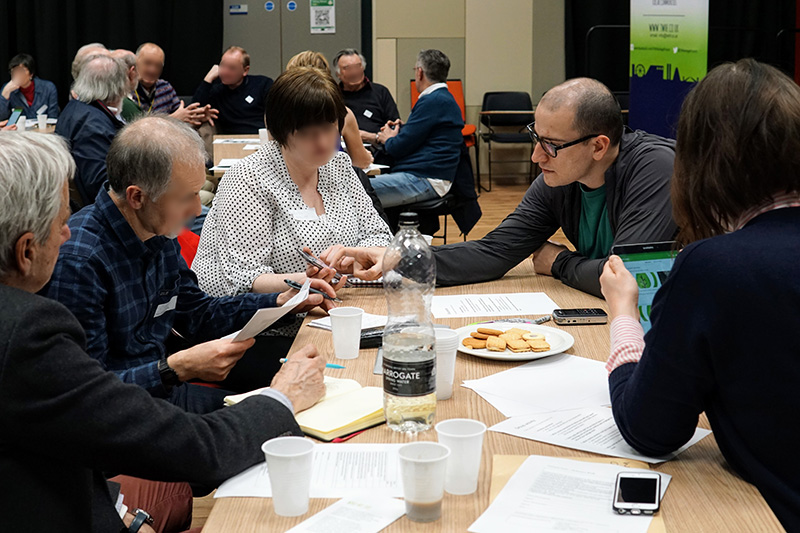
\includegraphics[width=0.9\columnwidth]{images/chapter06/HF_Workshop.jpg}
  \caption[The Heritage Forum ParkLearn workshop]{Participants discuss how they could utilise mobile learning apps during the Heritage Forum ParkLearn workshop.}~\label{fig:ParkLearnWorkshop}
\end{figure*}

While the participants agreed that they would prefer that the spaces be properly funded by local authorities, one reported positive outcome of volunteerism was the benefits that it can bring to the volunteers themselves. Several participants (of a variety of ages) talked about how volunteering in these spaces had given them opportunities for socialising, day-to-day structure and even boosted their self-confidence:

\begin{displayquote}
`Seeing what it's done for the volunteers as well has been fantastic. I started as someone who wasn't working, wasn't confident, and now my job is to have as much fun as possible down there.' 
\end{displayquote}

It's likely that these positive experiences have been a major contributing factor to the volunteers having such strong relationships with the places in which they volunteer. As these relationships developed, some found that they seemed to value the spaces more than other stakeholders---including the local government. This only seemed to change after the volunteers' work had started paying off:

\begin{displayquote}
`At one point it was something that the city council wanted nothing to do with, it was a liability for them. But now it generates a reasonable income, and wherever you go, people go "Ooh, I didn't know about that, it was great."' 
\end{displayquote}

However, one participant in her 20s argued that while she enjoyed volunteering, she had struggled to get other young people to join. She noted that while the austerity measures rely on volunteerism, many young people find the current economic environment too hostile to be able to afford to work unpaid: 

\begin{displayquote}
`There's a large student population in Newcastle, so we're trying to figure out how to cater to them, and how we secure the next generation of volunteers. Cos my generation can't really afford to volunteer---we can't really afford to pay rent, let alone volunteer. So, it's figuring out how we're gonna make it sustainable.
\end{displayquote}

This seems to point to an unfortunate situation where conservative policies (both fiscally and socially) have worked against each other: Big Society relied on volunteerism and local action by citizens, but stagnant wages and crippling austerity measures has meant that an increasing number of people are unable to afford to volunteer.

\subsubsection{Augmenting Space to Highlight Place}

These relationships with space also frequently appeared to come with an appreciation for the different ways in which these spaces had been used by different stakeholders over time, even in ways which would traditionally be seen as anti-social or even destructive. There seemed to be a desire to highlight these factors, potentially to share their value with others who might not immediately appreciate them. For example, one volunteer referred to the value of the area's graffiti, noting it as a part of the local heritage which could be shared through the ParkLearn app:

\begin{displayquote}
`We've got interpretation boards above ground, but they get covered in graffiti. [considers] ...We've also got a load of graffiti, and it would be amazing to have [the app] talk to it. We've got little bits of heritage all over the valley, and it would be amazing to tie this into that, so people could take more self-guided tours.'
\end{displayquote}

Similarly, the `imperfections' of space---typically signs of life from former stakeholders---were seen to add to the character of place. In a way, these pieces of evidence of how the spaces have been used over time form a new layer of place infrastructure, which evolves over time and helps give each place unique identities and meaning. One of the participants noted concern about how making some of these spaces safe for public use could potentially sanitize these characteristics out of existence, creating a tension between encouraging greater use of space and preserving what makes it special:

\begin{displayquote}
`If we tried to secure funding and make parts of it accessible, it would actually lose quite a lot of its charm, its history. There's old bits of park benches still down there... there's graffiti not just from the war, but there's graffiti from when someone took a Margaret in for her birthday in 1968 and wrote on the wall about it. So it gets added to all the time, and we just go in periodically to check that no-one's died down there.'
\end{displayquote}

For these reasons, it may be important to consider where and when mobile learning interventions are suitable: while they may be useful as tools to highlight particular aspects of place which otherwise may go unrecognised or underappreciated (e.g. the graffiti), they may also be detrimental to the sense of place, or intrusive on the people who live there. For example, there may be elements of place which people may not want to be highlighted to outsiders. While Relph warned about the dangers of sanitisation leading to inauthentic, `Disneyfied' experiences \citep{Relph2018}, airing a community's dirty laundry should also not be done without any critical consideration of the potential consequences. Similarly, we should be aware of technology's impact on space, even when the content being highlighted to visitors is unlikely to be perceived as negative. An obvious recent example would be users of the Pok\'emon Go app intruding on private property and socially sensitive areas (such as historical landmarks and graveyards), to the point of a class action lawsuit being filed against its creators \citep{Marder2016}.

However, this doesn't mean that the use of mobile learning applications in community areas shouldn't be done when handled tactfully. One participant describes how a group worked with a local school and surrounding residents to create a history trail, with residents' houses being many of the points of interest:

\begin{displayquote}
`A group has created what they've called a poppy walk, where they've recorded the 400 World War One casualties that came from the town, and a hundred of their residences are still standing. They've put these resin, bronze poppies [on the buildings]. And they've created this app, so when you come to the property, it says `this is where lance corporal so and so lived, he was killed on...', and you get that. They did that with school children from a local secondary school.'
\end{displayquote}

In this instance, by working with homeowners the group were able to modify the physical elements of space in order to highlight properties of place, which could then be further explored through a mobile learning technology. Another participant went the opposite route, and used digital technologies to create their own layer of place infrastructure, which no one else could interfere with:

\begin{displayquote}
`We have only one blue [commemorative] plaque in the area, and we're looking to identify potential individuals, events or places that would warrant one. The idea I've come up with is to create virtual blue plaques---that way, I can create as many as I like, without arguing over `well I don't like him', and all the rest of it. So I'm obviously now thinking to put this app with it. So I'll go the virtual route first of all, that way I can create as many as I like, and then present them to the local population to ask who they want as a physical plaque.'
\end{displayquote}

The participant noted that due to the passage of time, the space being augmented may have significantly diverged from the space that existed at the time of the heritage being highlighted:

\begin{displayquote}
`The issue with a new build town, is that you don't have the buildings to put [commemorative plaques] on. So if you find someone who was important in 1850, well... where he was important is now long gone.'
\end{displayquote}

While the physical commemorative plaques were limited by such changes, the non-corporeal nature of digital installations meant that the digital versions---which were fully under the participant's control---would be able to be deployed, regardless of the current state of the space in question. In this regard, having digital authorship capabilities gave the participant an advantage in expressing their world-view and performing active citizenship.

However, some of the heritage which participants wanted to highlight would still be relevant to current versions of space and place, simply due to its influence upon the surrounding communities. For example, a participant suggested that the \textit{Record Audio} and \textit{Listen to Audio} Task Types could be used to share local music, originating from the 1984-1985 miners' strikes:

\begin{displayquote}
`For example, I'm a song writer. We could have had people sing songs into that app. And then they could have cited where the song originated, and stuff around the miners' strike, things like that.'
\end{displayquote}

These strikes were hugely divisive at the time, and the subsequent closing of the mines resulted in many impoverished communities. These events were clearly hugely influential on many places as they exist today, and so stand as an important part of their heritage. That said, the issue remains extremely emotional to this day (a murder in 2004 was claimed to be the result of an argument about the strikes \citep{theindependent_2004}, and many of the pro-strike areas voted heavily to leave the European Union in the 2016 `Brexit' referendum \citep{dailypost_2017}). Designers of technologies which support community-generated civic learning material should be aware that stakeholders may have strong and conflicting views on a place's social infrastructure. 

\subsubsection{Engagement and Sustainability}

Another key talking point was the importance of engagement with site visitors---be that the local community, tourism or schools. There were commonly negative opinions given of `traditional' styles of visitor engagement, such as interpretation boards (in-situ signs, displaying relevant text and images) and even traditional tour guides. There was recognition that while these styles of visitor engagement were often appreciated by enthusiasts, they were unlikely to engage new demographics:

\begin{displayquote}
`We have the interpretation boards, but people don't want to read reams and reams of text... Some people do, but you can cater for both.'
\end{displayquote}

These traditional engagements were seen as being particularly uninteresting to children, as they would want more varied and interactive elements, rather than being simply passive experiences:

\begin{displayquote}
`I was taken to a lot of historic sites when I was a child, but I was never really engaged with---I was just looking at things, reading things. There was no engagement.'
\end{displayquote}

Some of the participants' groups had reconfigured their previously traditional content to drive greater engagement with their space. One participant noted that their new style of tours helped ground the visitors' experiences of place, promoting empathy with the space's previous stakeholders through use of role-play and more interactive elements which brought the history `to life':

\begin{displayquote}
`It's so much fun---when I started, we had the two hour heritage tour and had the odd school group in. But now we're doing more things with props, dressing up, at Halloween we turn all the lights off... and they meet characters who lived and died in the area, so everything we do has that historical twist on it, and it means I get to run up and down the tunnel with a fake bottle of wee, spitting it at people. People like that grisly bit, so I like to make sure people leave thinking "I'm really glad I'm alive now, that I do the job I do now."'
\end{displayquote}

More common was a desire to embrace new digital technologies, and integrate them into the visitor experience. Having a digital presence was seen as particularly important for engaging with younger audiences and visiting schools:

\begin{displayquote}
`We've got social media and a website, we do loads of work with schools, and we're doing a lot more special events than we were. Trying to capture the younger demographic.'
\end{displayquote}

Beyond technologies such as social media and having a website (which were seen as being fairly attainable), several groups were looking for solutions for digital, in-situ experiences. These often would act as alternatives to the teaching materials (e.g. worksheets) usually offered by the sites to visiting schools. Solutions to this were seen as less obvious than simply having a web and social media presence, and several groups saw ParkLearn as a potential option for delivering interactive educational digital content:

\begin{displayquote}
`A lot of schools don't want worksheets, pen and paper. They want the kids to be more hands-on, interactive. But something like this, being able to record audio, take pictures... I'm actually trying to set up a geocaching, or map-type activity, so this could actually work really well. I've been struggling to find a way of delivering that sort of thing.'
\end{displayquote}

Several participants were inspired by how the park volunteers used audio recordings in their `Talking Statue'. They saw it as an opportunity to help bring their interpretation and exhibits to life in a manner similar to the other group's use of role-play, but without the need for staff to be on hand for every visitor. Furthermore, they hoped to provide a more authentic learning experience by providing audio recordings of the place's actual stakeholders:

\begin{displayquote}
`We're looking at this, and thinking instead of a tour guide talking, having this, be more interactive. Have the actual miners do the talking.'
\end{displayquote}

In a departure from these more passive learning experiences, one participant noted that a number of ParkLearn's available Task Types are more generative. They recognised that materials that students produced during site engagements could be used in classroom activities upon return to the school, as part of larger ongoing projects:

\begin{displayquote}
`If you were doing a project at the park, you could gather a lot of pictures, audio, whatever it might be, and if you can take that back to school you can use that as a basis of your project.'
\end{displayquote}

While there was a desire from many participants to have mobile learning technologies at their sites, there were also a couple of participants who noted concern over their sustainability. While several participants noted that the name `ParkLearn' was initially off-putting due to it seemingly being limited to use in local parks, there was a general appreciation of ParkLearn's generalisability, as it allowed groups to apply it to their own sites without the need for developing bespoke software (which many groups claimed not to be able to afford). For example, one participant recalled how a site's bespoke application---which had been hugely expensive to produce---had seen very little uptake by visitors, and viewed it as a waste of resources:

\begin{displayquote}
`I had to do something similar to this, and the company had already developed an app that they were using at another reservoir down south. It was all Beatrix Potter audio, video, stories for a walk around the reservoir, and it triggered as you walked around. And they spent... thousands developing this. Six people downloaded it.'
\end{displayquote}

On another table, a participant shared that their group were in meetings with software development studios, investigating how much a bespoke application aimed at engaging children with their project would cost:

\begin{displayquote}
`Our initial thought was to use augmented reality, and pick out 20 or so points of interest around the quay and develop an app. For example, you want to the statue that we just erected, point your phone at it, and all sorts of information would pop up---including audio, or pictures that would tell you how it was made, who built it, how the money was raised and that kind of thing. So this seemed like a good place to start, we had a couple of meetings about augmented reality. We know it will work, but it's quite pricey, expensive to develop. We were quoted around £30,000.'
\end{displayquote}

It was interesting to find that some groups were willing to risk such large amounts of money in order to create custom software, when it was unlikely that it would see much uptake. Particularly when an application is limited to working at a particular site, the amount of money spent per engaged user is likely to be relatively high. We were left speculating if engagement with the application itself was a secondary concern, and that having a bespoke piece of software (particular one with elements as `in vogue' as augmented or virtual reality) was more of a symbol of prestige for the more well-funded projects.

\subsubsection{Summary}
The findings of this workshop demonstrated to us that members of these groups frequently have a mutually beneficial relationship with the spaces in which they work---volunteers can be offered structure and opportunities for socialising, and places benefit from greater appreciation, leading to care and attention. However, the groups frequently had concerns around sustainability---austerity measures resulted in a move away from spaces receiving public funding, instead moving towards volunteerism. Furthermore, economic downturn has meant that groups are struggling to enlist volunteers from younger generations. In our previous studies, participants believed that nurturing peoples' relationships with a place would make them more likely to want to look after it. This would explain why so many groups were keen to directly appeal to younger audiences by digitally augmenting their spaces with mobile technologies. 

Some participants noted that by their nature, mobile learning technologies could highlight elements of place in a manner separate from the limitations of space. However, place does not always change as readily as space: events in a place's past---both positive and negative---can themselves form layers of infrastructure and contribute strongly to its identity. 

Many of the participants hoped that through mobile learning technologies, they could highlight underappreciated elements of place (e.g. value the graffiti as heritage), platform their values as community stakeholders (e.g. surface stories and songs from the miners' strikes), support more authentic engagements with place (e.g. listening to authentic placeholder accounts), and simply offer a more interactive visitor experience than what they could currently provide.

That said, concerns were raised with regards to the sustainability of implementing bespoke mobile learning technologies. For smaller, predominately volunteer-driven groups, creating a new piece of software was usually seen as unrealistic, due to the need for either technical know-how or substantial monetary investment. Furthermore, the adage of `build it and they will come' was reported to not always apply, making such investments a sizable risk. Several participants noted that the lower risk and cost of entry made generic solutions such as ParkLearn more appealing.

\subsubsection{Rebranding to OurPlace}
Following the concerns raised by several participants in this workshop, I decided to rebrand the platform. While `ParkLearn' was well suited for the previous engagements with park rangers and volunteers, the workshop highlighted that there was a demand for applications such as this in contexts other than parks. In these contexts, the ParkLearn branding was seen as off-putting due to its lack of contextual relevance, with many of these sites being urban or not associated with nature. 

\begin{figure*}
  \centering
  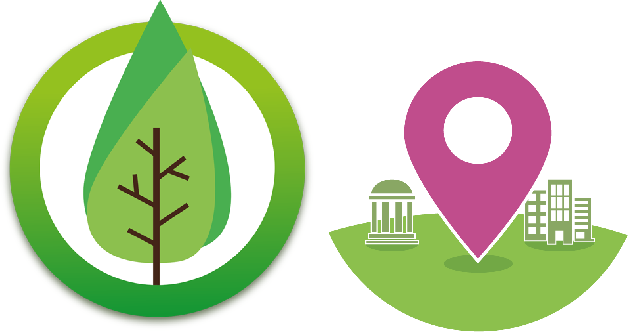
\includegraphics[width=0.8\columnwidth]{images/chapter06/logos.png}
  \caption[The ParkLearn and OurPlace Logos]{The ParkLearn logo (left) was updated updated to the OurPlace logo (right), moving focus away from nature and instead onto people's lived experiences in place.}~\label{fig:AppLogos}
\end{figure*}

Eventually the name `OurPlace' was settled upon, to reflect the platform's focus on enabling stakeholders to share their interpretations of place with others. It also moved the platform away from being explicitly about education, which may encourage older audiences to engage, who might have otherwise written it off as for children. The application's colour scheme and logo were updated, moving away from the previous brand's focus on nature and towards one which instead focused on the lived environment (Figure \ref{fig:AppLogos}).

\subsection{Heritage Forum Conference, OurPlace Workshop}
\label{sec:HeritageOurPlaceWorkshop}

I also held a short workshop at the Heritage Forum's conference the following year. This workshop consisted of a short presentation introducing the project, and then an interactive section in which participants were able to try out the OurPlace app for themselves. I had pre-prepared an Activity about the conference venue, and loaded it onto the available tablets. The Activity was designed to show how the app could be used both as a form of digital interpretation and as way to provide visitors with a more interactive experience. As the Activity was limited to being inside the venue, I chose not to use \textit{Location Hunt} Tasks. Instead, the Activity guided the participants around to different areas of the building to find various QR codes, which when scanned revealed information about its heritage and various interactions as Follow-Up Tasks.

While short, this workshop highlighted how varied the levels of digital literacy can be, even amongst people of similar demographics. For example, a representative from one heritage group was interested in if they could run their own version of the OurPlace server, offline on their local network---their site was a cave system, and didn't have access to the Internet. This person clearly had technical knowledge, as they were asking about how they could use the open-source nature of OurPlace to make it more suitable to their own circumstances. However, in the same workshop were multiple individuals who had never used an app, or seemingly even held a smart device before. It was clear that I had over-estimated the base technical literacy of the participant group, as this person was asking me to explain what a smartphone app was---while the app's documentation had explained some basic information for non-technical users (e.g. how to download the app from Google Play), it was within with an assumed base level of knowledge about the \textit{existence} of the technologies and interface metaphors the app is built upon. Accommodating both of these potential audiences was extremely difficult in the workshop, but it was clear that the many of audiences that the app was targeting (i.e. heritage enthusiasts, institutions and volunteer groups) would also be comprised of individuals with a similar mix of degrees of comfort when dealing with technology.

\section{Use of OurPlace by Community Groups}

Following the Heritage Forum workshops, several groups were interested in using the OurPlace app at their sites. While a number of these groups did not end up using OurPlace at their sites, several did adopt the app and created their own Activities. This section will give some brief examples of how the OurPlace app has been successfully used by various community groups to promote the places in which they operate.

\subsection{Lighthouse}

Operated by the local Council, this lighthouse is a local tourist attraction, offering a gift shop, nature reserve and paid entry into the lighthouse itself. This Activity's existence was a particular surprise, as I found it by coincidence while visiting the lighthouse. Having attended the heritage workshop, the lighthouse's staff had soon afterwards independently downloaded OurPlace and created their own Activity for visitors to use. Rather than focus on the lighthouse's history, the creators seemed to be more interested in creating an entertaining activity for visitors: consisting entirely of \textit{Photo Match} Tasks, this Activity simply challenged its users to explore the lighthouse, and find particular features within the space.

\begin{figure*}
  \centering
  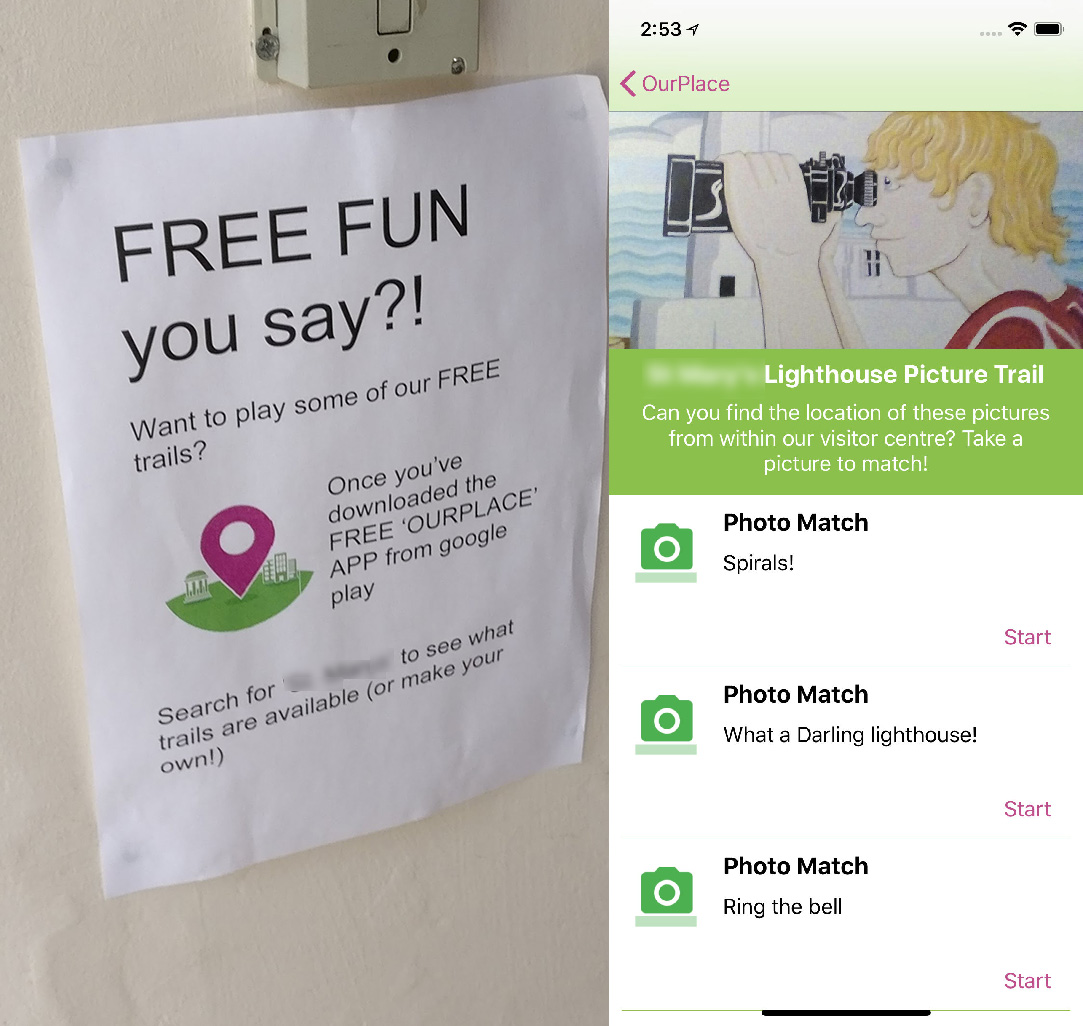
\includegraphics[width=0.65\columnwidth]{images/chapter06/OurPlaceLighthouse.jpg}
  \caption[An OurPlace Activity at a lighthouse]{The management of a lighthouse visitor centre advertise their OurPlace Activity, and invite visitors to make their own.}~\label{fig:OurPlaceLighthouse}
\end{figure*}

The Activity's creators went as far as to create their own poster, advertising the existence of the Activity and featuring the OurPlace branding (Figure \ref{fig:OurPlaceLighthouse}). However, they clearly misinterpreted the app's Activity discovery system: the poster tells users to search for the lighthouse's name, rather than the Activity's share code. The creator also either didn't know about the QR code scanning feature or the app's website, as the poster also doesn't feature the Activity's QR code. 

One interesting thing to note is the poster's call to action, suggesting that visitors create their own Activities around the lighthouse. While some other groups had been hesitant about the idea of anyone being able to create Activities in their space, the lighthouse creator seemed to welcome public contributions and collaboration.

\subsection{Railway Museum}

Designed to transport coals from the region's pits, this site features one of the world's earliest modern railways. As well as the railway lines and several restored locomotives, it boasts a small museum, with a gift shop and tearoom, ran largely by volunteers. One of the site's staff (HP1) was a Heritage Forum member, and wanted to create a walking trail around the site using the OurPlace app.

Initially, HP1 wanted to create a `premium' OurPlace Activity to coincide with a major regional event, which was expected to attract a large number of tourists into the area. The museum had been given access to some funding to take part in the event, and they wished to commission the creation of premium assets to be used in an OurPlace trail. This included audio interviews from local stakeholders, photos from the site and cartoons relating to the site's history. However, HP1 seemed to have a misunderstanding of how the app actually worked: rather than Activities being structured sets of Tasks into which you put content, they thought it was something more akin to a fully customisable website, where creators could change how the app looked and behaved. This confusion, which seemed to stem from the participant's lack of experience with the app and low technical literacy, resulted in the Activity not being made in time for the event.

However, once this confusion had been cleared up, HP1 realised that creating OurPlace content was also less technically demanding than they had originally thought. As they were still uncomfortable with creating an Activity independently, I agreed to assist in making it with them on their iPad device. This resulted in a digitised version of a previously existing trail, using \textit{Location Hunt} Tasks to guide the user between points of interest. Each point of interest had an \textit{Information} Task associated with it, featuring some written information about the location's history and some historical photos. The Activity was made public, and made available to launch from QR codes within the site's museum or by its association with the site's location in the OurPlace app.

\subsection{Modern Art Trail}
\label{sec:ModernArtTrail}

I was contacted by a retired art teacher (HP2), who had recently started volunteering to run tours of the modern art pieces installed in a local park. They had found out about OurPlace through the Talking Statue installation, and wanted to know how suitable the app would be for use as part of their art trail. After discussing the app and going around the trail, HP2 decided to go ahead with creating an Activity. However, as they didn't own a smartphone and weren't very comfortable with using digital technologies independently, they arranged a follow-up meeting for other members of the park's \textit{Friends} group to attend.

\begin{figure*}
  \centering
  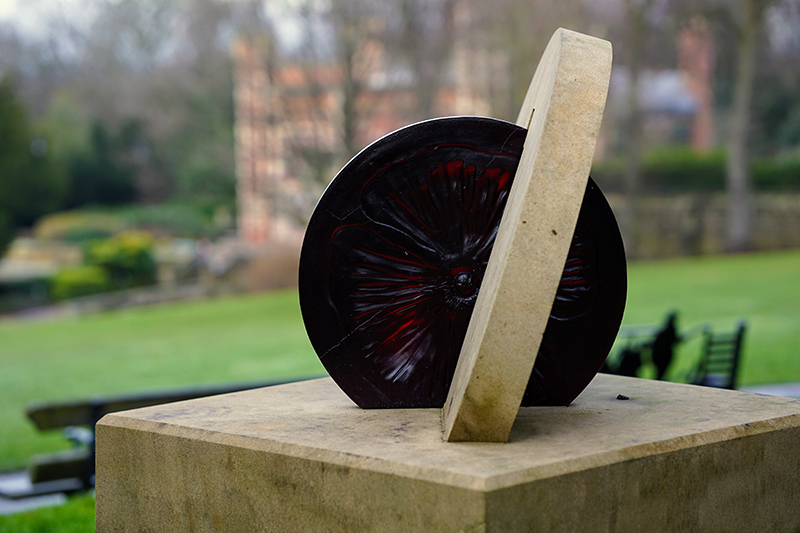
\includegraphics[width=0.7\columnwidth]{images/chapter06/artpiece.jpg}
  \caption[An art piece which was used in an OurPlace Task]{Users of the art trail Activity were challenged to catch the sun's light through this glass poppy, and reflect on how the piece would be altered by different light conditions.}~\label{fig:ParkArt}
\end{figure*}

This meeting took place in a function room in one of the park's main buildings. To assist the group in designing the OurPlace Activity, I took along a jigsaw kit (described in Section \ref{sec:PrototypeWorkshop}) so that they could start designing a paper prototype of the Activity without having to be completely comfortable with the digital interface. After a brief demonstration of the app, the participants started outlining and discussing an Activity using the jigsaw and HP2's notes about the different art pieces, which included blurbs about the artists and the reported meanings of the pieces themselves. 

Rather than be a simple trail which passively delivers information at each stop, the group were interested in how they could use the different functions of the app to enhance the visitor's experiences with the artwork. For example, suggested Tasks included challenging the user to \textit{Take a Photo} of the sun's light passing through the glass of a particular sculpture (Figure \ref{fig:ParkArt}), and then \textit{Record Audio} reflecting on how they think the mood of the piece might change in a different light. Because the trail was becoming so generative, the participants became interested in how they could use people's uploaded responses: ideas included featuring them on the \textit{Friends} group's website, and creating collages of the uploaded images. Because of this, the group were keen on creating the Activity on their own devices, so that they could view authorised responses on the website. They were also concerned about the privacy settings for those who responded, but were satisfied with how the app handles privacy settings once they were clarified.

\begin{figure*}
  \centering
  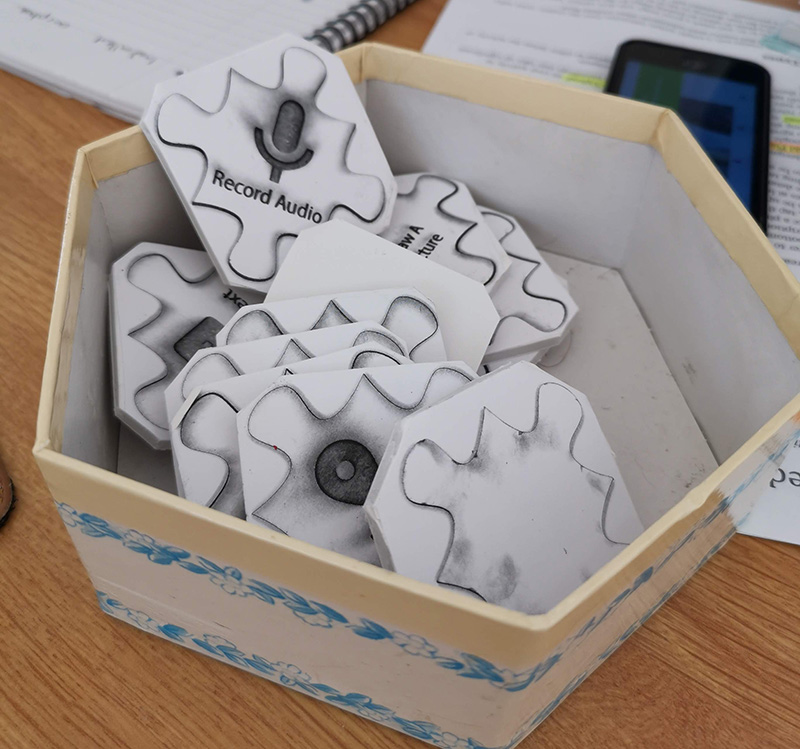
\includegraphics[width=0.65\columnwidth]{images/chapter06/DIY_jigsaws.jpg}
  \caption[Homemade jigsaw pieces created by a \textit{Friends} of the park group member.]{The homemade version of the jigsaw Task Type pieces, created by a member of the park's \textit{Friends} group to assist in designing Activities in the park.}~\label{fig:DIYJigsaw}
\end{figure*}

Rather than create the Activity there and then, the group decided that they wanted to take their time designing the Activity over several sessions, and were happy to do so independently. They claimed to find the jigsaw extremely helpful, and borrowed it to use in their design sessions. Having been able to get used to the structure of the app's Activities through the jigsaw, HP2 now felt more comfortable with the idea of engaging with the technology, and ordered their first smartphone so that they could work on the Activity at home.

Despite this added confidence, they still ran into a couple of issues with the application and asked for help through a follow-up meeting (it turned out they had mixed up the \textit{Record Audio} and \textit{Listen to Audio} Task Types, and were confused as to how they could add audio files while creating \textit{Record Audio} Tasks). During this meeting, one of the members (HP3) revealed that they had created their own Task Type tokens by printing out images of the jigsaw pieces onto foamex board (Figure \ref{fig:DIYJigsaw}), and had been using them to further help them keep track of what Tasks they were creating for each Activity. While we created an Activity together on one of their own phones, HP3 laid these tokens out during the planning stage, and then flipped them over as the Tasks were created. In this way, the tokens acted as a simpler version of the jigsaw, as they didn't require the planning of the Task descriptions.

During this follow-up meeting, HP3 also noted that they had decided to create two versions of their trail: one for the visitors who would normally consider going on the trail anyway, and another version designed for use with schools. While the first one would largely be a digitised version of the existing trail's format, focused on the delivery of information (with some added interactions to stimulate reflection on the art pieces), the version designed for schools would make use of the seamless nature of the OurPlace application. This version would focus on the more creative and generative Task Types, with the explicit intention for students to generate materials and record their reflections in-situ for later use upon return to the classroom. When I enquired what had inspired them to use the app in this way, HP3 revealed that they had printed and been thoroughly (with the liberal use of highlighter) reading one of the project's resulting publications \citep{Richardson2018} of their own volition.

\subsection{Community Railway Partnership}

Another member of the Heritage Forum (HP3) got in touch to enquire about their potential use of OurPlace within their group's educational activities. HP3 was an officer in a `community rail partnership' (CRP) group---a not for profit company that works with train operating companies to `promote, strengthen and protect' the role of a particular railway line in the North of England. The group aims to increase public awareness of the rail services, increase community involvement in the rail lines and strengthen links between the railway industry and the communities and businesses it serves.

HP3 arranged to meet me at Open Lab, along with the CRP's Company Secretary and their Director of Finance, as well as the Community and Sustainability Manager for the railway line's train operating company (HP3 invited this person as they wanted them `\textit{to see that OurPlace could be a great community engagement tool for the Community Rail Partnerships in the North East}', but unfortunately they could not attend the meeting). The group were interested in how they could use mobile learning as a part of their delivery of educational activities on and around the railway. During the meeting I gave a demonstration of the OurPlace app by showing some example Activities (made by both adult stakeholders and school students [covered in Chapter \ref{chap:student-created}]), and the process of creating new ones. When conversation moved onto how children themselves could create Activities as a part of the educational events, I also demonstrated the jigsaw activity for creating paper prototypes of OurPlace Activities.

The group brainstormed several ideas about how they could use the OurPlace application to deliver engagements. Ideas included: i) creating Activities in the app which could be completed by visitors and children, both during train journeys and about particular stations (e.g. related to the history of stations and the railway---how they had been used, and how communities had formed around them); ii) children researching these and other subjects, and then creating their own Activities to share with peers and other railway users; iii) using OurPlace Activities as engagement platforms, through which communities could use different Task Types (e.g. \textit{Take a Photo},\textit{ Map Marking}) to engage with the CRP staff---e.g. providing evidence of volunteer work, or report issues with facilities. 

By the end of the meeting, the CRP group had decided that they wanted to use OurPlace as a major part of their engagement programme. The final portion of the meeting was consisted of them discussing the practicalities of what was needed to do so. For example, HP3 saw value in the jigsaw activity as a process for designing Activities (particularly with school groups), and was curious about how they could be made (to the extent that they asked if they could order kits for purchase from Open Lab). The other main considerations were device availability (tablets would have to be bought for the purpose of running OurPlace engagements), and the need to have staff who were i) trained in the use of the OurPlace platform ii) able to dedicate time to design, create and deliver educational sessions which made use of the application.

The group decided that they would apply for a number of grants from the train operating company, both in order to cover the costs of purchasing a number of tablets and to finance a member of staff who would be dedicated to designing and delivering OurPlace engagements for the CRP. At the time of writing, £17,000 of funding has been secured for this, with the CRP awaiting final confirmation and receipt of funds before proceeding in advertising the role.

\subsection{`Places in Transition' Study}

OurPlace was used in a separate research project (awaiting publication), led by Bobbie Bailey. The project aimed to explore how some of the technologies which have been blamed for the degradation of high streets and urban centres (through the changing of residents' economic and social habits---i.e. use of online shopping, social media, streaming video consumption) could be harnessed to highlight the value of these places, and encourage people to re-evaluate their relationships with them. The research team worked in collaboration with a particular Business Improvement District (BID): a non-profit organisation which aims to revitalise its local town centre by working in partnership with local businesses and the surrounding community, particularly focusing on culture through restoration efforts and the organisation of public events.

The research team co-created an OurPlace Activity with the BID, utilising the application as a medium to digitise the existing walking tours of the town centre which had been designed by a local community interest group. The research team note that the Activity acted as a technology probe, designed to `\textit{enable participants to contribute their own stories of [the town], with the aim of creating a platform for residents to express their civic pride and build upon people’s lived experiences and sense of attachment to place.}' Furthermore, they saw the use of OurPlace as an example of how the BID could use existing technologies to create discussion and raise awareness around local assets, and how such technologies could help nurture place-making between residents and their local urban centre.

The app's \textit{Photo Match} Task Type was utilised by the BID to contextualise the future development of the area, visualising planning decisions using basic augmented reality. The research team posited that this could be developed further to allow residents to contribute their own opinions and visions of the area's development. The researchers also found that the BID saw opportunity in OurPlace as a way of promoting experience-led approaches, engaging people during cultural events and highlighting the town's assets. The application's location-based Task Types were seen as being particularly valuable, with the Activity making use of \textit{Location Hunt} and Follow-Up Tasks to highlight local history and attractions in a more interactive and `fun' way. The Activity also used a \textit{Map Marking} Task, challenging people to discover parts of the town that were seldom visited. This Task's description read:

\begin{displayquote}
`Find at least 5 of [the town]'s many hidden alleys, yards and small streets! There are loads of small lanes, yards and alleyways and streets in [the town] to discover, all with their own unique charm and are full of wonderful independent shops, bars and restaurants. Rediscover as many as you can!'
\end{displayquote}

In this way, the BID saw the digital tools such as OurPlace as a way to provide modern ways to highlight forgotten place assets to the local community. They perceived that modern solutions to these issues required the use of digital tools, noting that technology is something that they `\textit{would have to use}'. They also believed that it could help with engaging with younger generations, and hoped that these generations would go on to value and take care of the town centre. Furthermore, OurPlace was seen as more economically viable than manually running tours, as it didn't rely on the availability of an expert to conduct it.

\section{Discussion: Stakeholder Desires, Requirements and Tensions}

While the stakeholders that these studies engaged with worked within a wide variety of physical contexts (including mines, lighthouses, museums and parks) and roles (from volunteers, to tour guides and IT managers), they shared a relatively common set of desires---engaging with new (and particularly younger) audiences. This commonality of agendas aligns with the findings of Chapter \ref{chap:DesignSpace}, where the park rangers were keen to demonstrate the civic value of the places they cared about to new visitors. There was a hope that by giving visitors an appreciation for their spaces and the work that goes into maintaining them, visitors would gain some sense of ownership and responsibility for them, perhaps even leading into active participation in their upkeep, if not passive support. Of course, the most sustainable route to this would be for younger generations to become place stakeholders, ensuring that the places would be supported in the future. Many of the groups that we engaged with saw mobile technology as a promising entryway to engaging and encouraging place-making in younger audiences. For example, several participants mentioned how they had noticed that Pok\'emon Go had brought new audiences to their sites, and had been looking at how they could utilise similar technologies to engage with elements of \textit{place} as well as space.

However, practicalities frequently came between these community groups and the integration of technology into their sites. For example, by their nature some spaces were fragile or socially sensitive, and couldn't support permanent signage for interpretation or QR codes. Additionally, there was a large variation in the degree of technical literacy that could be found in each group. While some were clearly comfortable with digital technology, others had very little experience and were reluctant to even try engaging, limiting their representation in any created digital artefacts.

The groups we engaged with also had a wide variation in the amount of funding they had access to. While some groups were in a position to be able to consider spending significant amounts of money, others were asking the volunteers to contribute towards tea and biscuits. This affected everything from access to smart devices (e.g. could visiting school groups be supplied with tablets?) to the creation of the software itself. In some groups, there also seemed to be a lack of critical assessment in how the introduction of technology would benefit their project. On the most extreme end of this was the group considering funding the development of a premium application full of cutting-edge technology at the cost of £30,000. It wasn't clear why the participants thought these expensive features would be necessary, leading me to speculate that they viewed the adoption of these technologies as a sort of status symbol, differentiating them from other sites. They also placed a clear value on the use of bespoke applications rather than existing platforms, enough to warrant the costs of development. An interesting point was that those that were placing the most value in acquiring a bespoke system were not necessarily the ones with the most technical knowledge (e.g. the participant enquiring about running a version of the OurPlace server on their own offline network). While the desire to have a personalised, bespoke application is understandable, funding it presents a sizable risk to these small groups, or at least a strange value proposition: the number of visitors who are likely to search for, install and engage with an application that only works at one (small to medium sized) site is likely to be fairly small (or tiny---one workshop participant reported that only six people downloaded their site's augmented reality application, even though it cost thousands to develop). The groups' perceived need to integrate mobile technology and the potential lack of visitor engagement with it existed as a tension, one that most groups managed by simply minimising the amount of financial risk they were exposed to.

Another factor of interest was the interconnected, three-way relationship between technology, place, and the physical space that the groups worked within. Some of these existed simply as space presenting logistical issues (e.g. not being able to get mobile signal at a remote site) which would affect the performance of the technology, leading to the need for workarounds such as pre-loading content or running local servers. More interestingly, however, it was noted that technology can also be used to subvert the relationship between space and place. For example, when discussing the installation of commemorative plaques, one participant pointed out that in the context of heritage space changes over time, to the point where it may no longer reflect the memories of place. In this instance, the participant saw an opportunity for technology to highlight these properties of place through digital plaques---as they would exist independent of physical space, they are not limited by it. Finally, we found that several groups were hesitant about the open nature of the OurPlace app, and didn't like the idea that anyone could create Activities about their spaces. These groups felt protective over their site's image and reputation, and weren't comfortable with not being in control of all digital materials that were associated with their site. This hints towards an interesting tension between the `official' interpretations of place and those of the surrounding community, and how digital mediums can decouple the ownership and control of space and place. This was again reflected in the creation of commemorative plaques---the participant was able to subvert the usual channels and create their own plaques in a digital medium, taking control of the process without the need for choices to be sanctioned by the community.  

Finally, the `Places in Transition' study also highlighted the potential for mobile learning technologies such as OurPlace to be seen as `replacements' for the more expensive in-person interactions with community experts. While this could also be argued to be a factor in the app's usage in the modern art trail, in that case the technology was seen as a supplementary tool, which could either augment the existing tour or act as a back-up should the guide not be available. As I noted in Section \ref{sec:DigitalCivics}, there exists a danger that tools designed to support communities coping with austerity measures could be utilised in a manner which supports the austerity measures themselves: propping them up by taking pressure off of public services through the use of volunteerism, automation and DIY approaches. The potential for OurPlace to be used in this way is regrettable, but unfortunately I can't see a way around it. Instead, I can only promote the ways that the application has been used by these participants as intended: giving stakeholders new platforms for sharing their value of place, highlighting local resources and assets in ways which can appeal to new audiences.

\section{Summary}
This research highlighted how place stakeholders perceived a need to utilise new (particularly mobile) digital technologies to attract new, younger audiences---typically in an effort to promote place-making and, eventually, volunteering. However, due to ongoing social contexts, these stakeholders typically existed as volunteer groups with little funding and technical expertise. By their nature, if these volunteer groups had any digital assets (e.g. website), they were also frequently dependant on a core set of specialised individual members, with little planning for sustainability with skill sharing and duplication.

As such, many were receptive to using low cost, approachable and non-destructive `off the shelf' solutions such as OurPlace to share their knowledge and platform their agendas as place stakeholders. An example of this was shown in the `Talking Statue' deployment, where local volunteers used ParkLearn to have a statue narrate their park's history and highlight the work of the volunteer group. Through ParkLearn, the volunteers were able to take control of the process, independently creating a digital multimedia instalment with minimal interaction or financial support from the local council. Multiple other heritage groups made their own OurPlace Activities for similar reasons.

Analysis of participant discussions held during Heritage Forum engagements resulted in the development of several themes: `\textit{volunteerism and ownership of place}' (where volunteering tended to be mutually beneficial for both the place and the volunteer, leading to strong place attachment), `\textit{augmenting space to highlight place}' (using technology in space to highlight the value of place, particularly elements which are underappreciated, problematic or controversial) and `\textit{engagement and sustainability}' (the recognised need for engaging new audiences in ways which are more exciting yet still affordable, with the eventual goal of acquiring new volunteers). Finally, further reflections noted the prestige attached to the integration of cutting edge technology in sites (regardless of it being a questionable value proposition), and issues surrounding the interconnected, three-way relationship between technology, place, and physical space: where the degrees of separation between the three prompted questions of ownership, and allowed for the subversion of space when reflecting upon place.